%% IEEE Transactions Skeleton File
%% for students 
%%
%% Julian Zobel, Marcel Mann
%% Technische Universitaet Darmstadt
%%
%% v1.1 --- 08.07.2019
%%
%% 	Based on:
%% 		bare_conf.tex
%% 		V1.4b 2015/08/26
%% 		by Michael Shell
%% 		See: http://www.michaelshell.org/ for current contact information.



\documentclass[conference]{IEEEtran}

\usepackage{color}

\usepackage[utf8]{inputenc}

%%============================================
% FOR A DOCUMENT IN GERMAN! (Easy Umlaute etc)
%============================================
% \usepackage[american,ngerman]{babel}


%%============================================
% GRAPHICS (including path and extension declaration)
%============================================
\usepackage[pdftex]{graphicx}
% declare the path(s) where your graphic files are
\graphicspath{{./pics/}}
% and their extensions so you won't have to specify these with
% every instance of \includegraphics
\DeclareGraphicsExtensions{.pdf,.jpeg,.png,.jpg}

\usepackage{subcaption}
\usepackage{hyperref}

%============================================
% CITATION
%============================================
\usepackage{cite}
% cite.sty was written by Donald Arseneau
% V1.6 and later of IEEEtran pre-defines the format of the cite.sty package
% \cite{} output to follow that of the IEEE. Loading the cite package will
% result in citation numbers being automatically sorted and properly
% "compressed/ranged". e.g., [1], [9], [2], [7], [5], [6] without using
% cite.sty will become [1], [2], [5]--[7], [9] using cite.sty. cite.sty's
% \cite will automatically add leading space, if needed. Use cite.sty's
% noadjust option (cite.sty V3.8 and later) if you want to turn this off
% such as if a citation ever needs to be enclosed in parenthesis.
% cite.sty is already installed on most LaTeX systems. Be sure and use
% version 5.0 (2009-03-20) and later if using hyperref.sty.
% The latest version can be obtained at:
% http://www.ctan.org/pkg/cite
% The documentation is contained in the cite.sty file itself.


%============================================
% MATH
%============================================
\usepackage[cmex10]{amsmath}
% A popular package from the American Mathematical Society that provides
% many useful and powerful commands for dealing with mathematics.
%
% Note that the amsmath package sets \interdisplaylinepenalty to 10000
% thus preventing page breaks from occurring within multiline equations. Use:
%\interdisplaylinepenalty=2500
% after loading amsmath to restore such page breaks as IEEEtran.cls normally
% does. amsmath.sty is already installed on most LaTeX systems. The latest
% version and documentation can be obtained at:
% http://www.ctan.org/pkg/amsmath


%============================================
% FLOAT
%============================================
\usepackage{fixltx2e}
% fixltx2e, the successor to the earlier fix2col.sty, was written by
% Frank Mittelbach and David Carlisle. This package corrects a few problems
% in the LaTeX2e kernel, the most notable of which is that in current
% LaTeX2e releases, the ordering of single and double column floats is not
% guaranteed to be preserved. Thus, an unpatched LaTeX2e can allow a
% single column figure to be placed prior to an earlier double column
% figure.
% Be aware that LaTeX2e kernels dated 2015 and later have fixltx2e.sty's
% corrections already built into the system in which case a warning will
% be issued if an attempt is made to load fixltx2e.sty as it is no longer
% needed.
% The latest version and documentation can be found at:
% http://www.ctan.org/pkg/fixltx2e


% correct bad hyphenation here
\hyphenation{op-tical net-works semi-conduc-tor}
\hyphenation{data-base}


%============================================
% Notes and Annotations
%============================================
\usepackage{lipsum}                     % Dummytext
\usepackage{xargs}                      % Use more than one optional parameter in a new commands
\usepackage[pdftex,dvipsnames]{xcolor}  % Coloured text etc.
% 
\usepackage[colorinlistoftodos,prependcaption]{todonotes}  % , textsize=tiny
\newcommandx{\unsure}[2][1=]{\todo[		inline,	linecolor=red,			backgroundcolor=red!25,			bordercolor=red,#1]{UNSURE: #2}}
\newcommandx{\change}[2][1=]{\todo[		inline,	linecolor=blue,			backgroundcolor=blue!25,		bordercolor=blue,#1]{CHANGE: #2}}
\newcommandx{\notes}[2][1=]{\todo[		inline,	linecolor=yellow,		backgroundcolor=yellow!25,		bordercolor=yellow,#1]{NOTE: #2}}
\newcommandx{\add}[2][1=]{\todo	[		inline,	linecolor=OliveGreen,	backgroundcolor=OliveGreen!25,	bordercolor=OliveGreen,#1]{ADD: #2}}
\newcommandx{\improvement}[2][1=]{\todo[inline,	linecolor=Plum,			backgroundcolor=Plum!25,		bordercolor=Plum,#1]{IMPROVE: #2}}
\newcommandx{\noshow}[2][1=]{\todo[disable,#1]{#2}}

\begin{document}
%
% paper title
% Titles are generally capitalized except for words such as a, an, and, as,
% at, but, by, for, in, nor, of, on, or, the, to and up, which are usually
% not capitalized unless they are the first or last word of the title.
% Linebreaks \\ can be used within to get better formatting as desired.
% Do not put math or special symbols in the title.
\title{Scheduling Algorithms Optimizations in IEEE802.1Qbv Time-Sensitive-Networks}


% author names and affiliations
% use a multiple column layout for up to three different
% affiliations
\author{
	\IEEEauthorblockN{Saumya Jha}
	\IEEEauthorblockA{saumya.jha@stud.tu-darmstadt.de}
\and
	\IEEEauthorblockN{Yang Shan}
	\IEEEauthorblockA{yang.shan@stud.tu-darmstadt.de}
}
% conference papers do not typically use \thanks and this command
% is locked out in conference mode. If really needed, such as for
% the acknowledgment of grants, issue a \IEEEoverridecommandlockouts
% after \documentclass

% use for special paper notices
\IEEEspecialpapernotice{
	Technische Universit\"at Darmstadt \\
	Multimedia Communications Seminar II, Summer Term 2021
}

% make the title area
\maketitle

% As a general rule, do not put math, special symbols or citations
% in the abstract
\begin{abstract}

With the continuous development of the network, and the increasing demand for lower-latency and less-jitters real-time communication, Time-Sensitive Networking(TSN) is a new technology on deterministic transmission of network traffic, which has aroused widespread concern in both academia and industry. Moreover, there is the IEEE802.1Qbv enhancement to traffic scheduling, one of the core characteristic of the TSN is Time Aware Shaper(TAS), using a gate to enable or disable the transmission of the streams following a periodic schedule in the network. In this paper, we introduce the two general scheduling algorithms based on that, respectively Integer Linear Programming(ILP) and Satisfiability Modulo Theories (SMT). We address how the multi-hop switched network transfers the frames and chooses the scheduled/non-scheduled queues according to the Priority Code Point(PCP) in the 802.1Q header of the frames. Furthermore, several optimization approaches are proposed under two algorithms mentioned before, we compare the performance of these approaches to evaluate the practical effects.
\end{abstract}


\section{Introduction/Background
} \label{introduction}
% Now introduce the topic and motivate the research.
% Introduce the basic knowledge about Time Sensitive Network and 802.1Qbv.

% It presents the fundamental concepts of the paper. It starts with an overview of Time-sensitive Networks(TSN) followed by a discussion on IEEE 802.1Qbv standard. 

Industrial Internet applications have high requirements for real-time network transmission. Traditional Ethernet technology can no longer meet the real-time requirements of industrial Internet for data transmission. The emergence of time-sensitive network technology is expected to solve this problem.
 
Initially, in order to meet the needs of real-time, low latency, and de-jitter in audio/video transmission, the IEEE group established the AVB (Audio Video Bridging, audio/video bridge) group which is dedicated to improving the traditional Ethernet protocol. In 2012, the team officially changed its name to TSN (TimeSensitive Network). The time-sensitive network is composed of a series of protocol standards, including three standards for clock synchronization, data scheduling, and network configuration, so as to ensure the low latency and high reliability of the network. Since the time-sensitive network is based on the data link layer technology and has nothing to do with the upper-layer network protocol, it can theoretically be deployed in any network environment using Ethernet technology. For example, IEEE802.1AS is for Timing and Synchronization, IEEE802.Qbu is for Frame Preemption. Among these protocol standards, we will analyze and optimize IEEE802.1Qbv, which is Enhancements for Scheduled Traffic. 

For a typical TSN Switch, it contains multiple input(ingress) and output(egress) ports. For each output port, there are up to 8 FIFO queues connected to it. In a TSN network, different messages can be assigned different priorities according to requirements. When Ethernet frames of different priorities arrive at the TSN Switch, they will be assigned to different queues. The TSN Switch supports priority-based scheduling to ensure that high-priority queues are processed first. This priority-based scheduling has great advantages for high-priority Ethernet frames, but it is very unfair for low-priority Ethernet frames, because it may be blocked by high-priority Ethernet frames, and it can’t be dealt with for a long time. 

IEEE 802.1Qbv time-aware queues enable TSN switches to control queued traffic through a Time Aware Shaper (TAS). Ethernet frames are identified and assigned to VLAN tags based on priority. Each queue is Defined in a schedule, and then these data queue messages are transmitted at the exit within a predetermined time window. Other queues will be locked in the specified time window. Therefore, the effect of periodic data being affected by non-periodic data is eliminated. This means that the delay of each switch is deterministic and knowable. The data message delay in the TSN network is guaranteed.

TAS introduces the concept of a transmission gate, which has two states of "open" and "closed". When transmitting the selection process-select only those messages whose data queue gate is "open". TAS guarantees that queues with strict time requirements are protected from interference from other network information. It may not bring the best bandwidth usage and minimum communication delay. When the priority is very high, the preemption mechanism can be used. IEEE 802.1Qbv is mainly designed for those time-critical applications, which must ensure very low jitter and delay. IEEE 802.1Qbv ensures the transmission of real-time data and the exchange of other non-real-time data.

In section II we introduce the network and traffic model and formulate the scheduling constraints for IEEE 802.1Qbv. In section III we elaborate an SMT-based and ILP-based algorithm implementing the previously defined constraints together with a discussion and formalization of several optimization. We evaluate the scalability of our approach in section IV and survey related work in section V. We conclude the paper in section VI.

\section{System Model and Scheduling Approaches}
 %It gives an overview of the related scheduling methods used in the paper.
\subsection{System Model}

A Time Sensitive Flow is a stream of scheduled traffic, specified by a source, a destination, a period and the amount of data sent each cycle. We will also refer to time sensitive flow as flow. The source of a flow is the end-system injecting the traffic. The destination is the traffic’s targeted end-system that is to be reached. The period specifies the cycle time of the flow. The amount of data sent each cycle directly dictates how many time slots are required for the transmission of the data each cycle. We therefore model time as slots where each slot is capable of transmitting one frame of data. Every time-sensitive flow also has specified real-time guarantees associated with it that our joint routing and scheduling has to ensure. For this work we assume jitter to be within reasonable bounds and to not impact the schedules we compute, and we therefore neglect it. The real-time guarantees provided are that of ensuring frames get transmitted within a specified end-to-end delay.

Formally the topology of a network is defined by an directed graph $G(V, E)$, where the vertices V represent the hosts and switches, and the edges $E \subseteq V \times V$ represent the physical communication channels. Since the communication channels are full-duplex, every communication channel has to be represented by two edges: A channel which connects $v \in V$ to $u \in V$ is represented by $(u, v) \in E$ and $(v, u) \in E$.
 The set of streams is denoted as $S$. A stream  $s_k \in S$ defined by a 4-tuple: $s_k = ( s_k.src, s_k.dst, s_k.size, s_k.l)$ $s_k.size \in [64,MTU]$, $s_k.l \in [0,cycle\_time]$  
$s_k.src \in V$ is the flow’s source at which the frames get injected into the network. $s_k.dst \in V$ is the flow’s destination to which the frames get transmitted to. The stream $size$ is number of bytes and $l$ is maximum tolerated latency.

we model store-and-forward switching and cut-through switching. For store-and-forward, the frame needs to be completely received before the switch starts the processing of the frame whereas, for cut-through switching, only sufficient bytes need to be received to start the processing. In this paper, we assume the first 24 B containing the preamble, the Ethernet header, and the VLAN tag are sufficient to start the processing. 

The “Enhancements for scheduled traffic” allows for the implementation of up to eight queues to handle different types of traffic separately. The switch assigns a frame to one of the queues by evaluating the Priority Code Point (PCP) in the VLAN tag of the frame and a configurable mapping of PCP values to the hardware queues. 

Prioritization of data transmission is done on the egress port. A mechanism is needed to ensure that there is coordination between different data streams. A protection window is needed to ensure that high priority data has guaranteed access to the network at a specific instant in time. It can be created by allowing the transmission of a specific traffic class over a specific period of time. There are total 8 queues one for each traffic class to accommodate different traffic classes. Transmission is decided on the basis of algorithm known as Transmission Selection Algorithm(TSA). If the data from a particular queue is selected then the corresponding gate will be opened to transmit the data. Gate opening events are determined by gate control list. If there are fewer queues than eight, than data having multiple priorities can reside in a single queue. TSA decides in which order the data has to be transmitted from the queue. It has been shown in 
Fig 1. The gate following can block the transmission even though TSA has decided before the next opening gate event. This implies that we can give higher priority than the highest priority traffic type. The transmission algorithm can be selected on the basis First in First Out(FIFO) or it can be credit-based shaper(CBS) or vendor specific algorithm. So it is up to the industry to define the gate control list and how gates are operated. Gates control list is not needed if there are no enhancements to be made for traffic scheduling.

\begin{figure}[here]
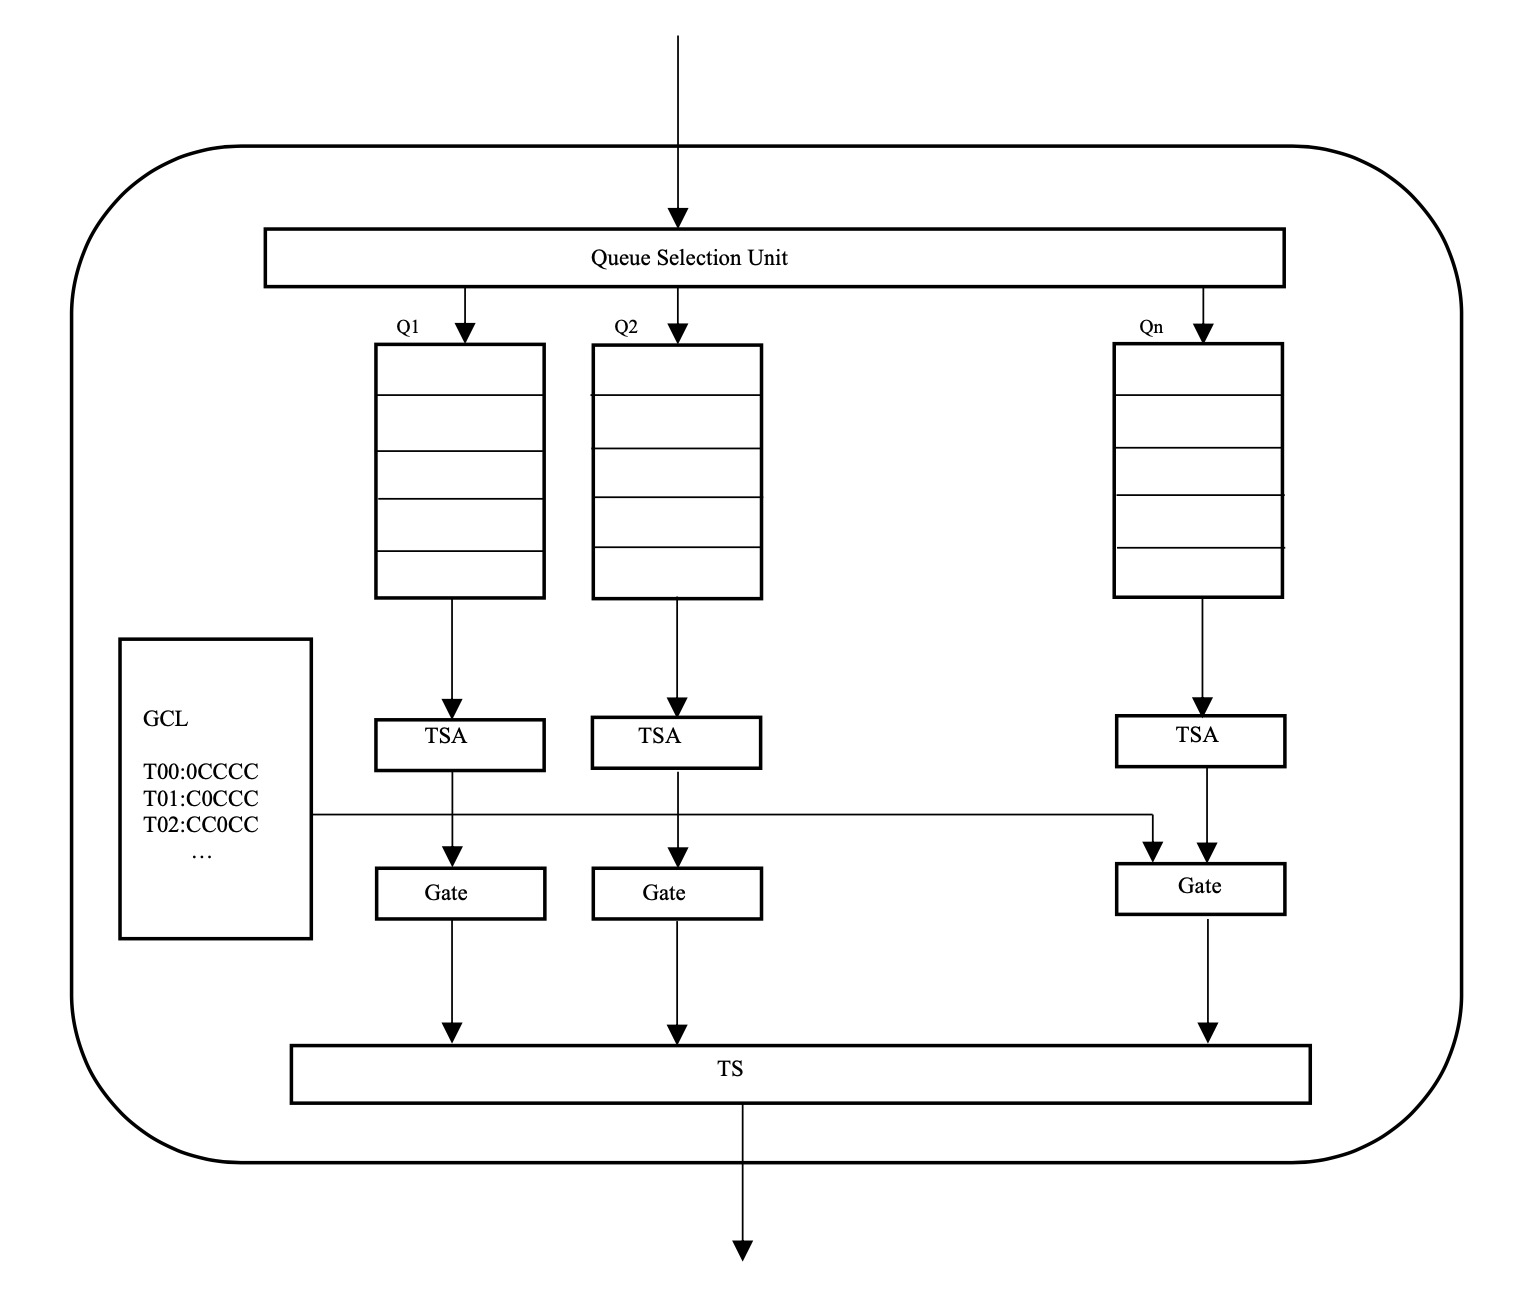
\includegraphics[width=9cm]{pic/figure_01.png}
\caption{Transmission Selection}
\end{figure}


\subsection{Integer Linear Programming(ILP) Solver}
% \textbf{Introduce the basic knowledge about Integer Linear Programming and the constraints.}

Linear programming (LP) is an optimization technique. Problems formulated as linear programs are optimized for a given linear objective-funktion while obiding given linear equality and linear inequality constraints. Integer Linear programming is like LP with the difference that some or all variables are restricted to be integers. ILP is NP-complete.

Typically there are clear optimization goals when formulating a schedule, for example minimizing average end-to-end delay of scheduled traffic. ILP solvers naturally lend themselves to these kinds of problems since they encorperate an optimization objective.
\subsubsection{Routing}

\subsubsection{Scheduling}

\subsection{Satisfiability Modulo Theories(SMT) Solver}
Introduce the basic knowledge about Satisfiability Modulo Theories and the constraints. 
\begin{itemize}
    \item[1)] Ethernet Specific Constraints
    \begin{itemize}
        \item[1.1)] Frame Constraint:It says that the frame offset of any scheduled flow must be equal or greater than 0. Also the entire transmission window has to fit within the frame period.
        \item[1.2)] Link Constraint: No two frames can overlap if they are routed on the same physical link in the time domain. ’item Flow Transmission Constraint: The propagation of the flows must follow the same order along the routed path of the flow. The constraint is set to individual frames rather than the complete flow instance as to allow the forwarding after the first frame has been fully received without waiting for the entire flow to buffer.
        \item[1.3)] End-to-end Constraint: It specifies that the difference between the arrival and sending time of a flow has to be within the specified maximum.
    \end{itemize}
    \item[2)] IEEE802.1Qbv Constraints
    \begin{itemize}
        \item[2.1)] Egress Interleaving: 
        It is to guarantee that the end-to-end latency is always fulfilled. The order in which the frames are placed in the scheduled queue is non-deterministic as schedule controls the gate opening events not the order of frames in the queue. This is due to some amount of synchronization error between different devices which may result in frames arriving not in order during runtime. It will result in accumulation of jitter for the overall end-to-end synchronization. This is not desirable when it accumulates with each hop along the flow path in hard real-time systems. This can be solved by guaranteeing the isolation of frames in the transmitting queues by a set of constraints. It can be done either by placing flows in different queues or the constraints must enforce some deterministic order of the flows in queues.
        \item[2.2)] Flow Isolation Constraint: In reality, it is not possible to achieve the ideal scenario due to frame losses or varying size of payloads over time.In such cases, deterministic behavior can’t be guaranteed as it can be seen with an example. Consider two frames are scheduled to arrive one after another from two different flows and placed accordingly in a queue at the switch. If one frame is lost than the other frame will take its place in the queue which can be transmitted in the original first frame time slot which leads to non-deterministic behavior. The constraint to enforce correct ordering of flows is that no frame is allowed to enter the queue until all the frames from the previous flows have been fully dispatched.
        \item[2.3)] Frame Isolation Constraint: The Flow Isolation Constraint is generally faster but it’s restrictive and may decrease the solution search space for valid schedules. In order to avoid this, the researchers relax the constraints to allow frames interleav- ing between flows in queues while same time guaranteeing the order on the egress port is deterministic. This can be achieved by allowing only frames of one flow in the queue at a time. If two frames from different flows have arrived than one can be allowed to enter in the shared queue if the other has already been dispatched from the queue.
    \end{itemize}
\end{itemize}

\section{Optimization}
Nice section. Do not forget to reference sources~. 
\subsection{ILP-based Optimization Algorithm}
% Presents the specification of the system model and the problem statement of paper 1. Presents the various scheduling algorithms that have been implemented in the paper 1. \cite{Craciunas2016}
\subsubsection{System Model}
%Introduce the system model and three approaches in the paper 1. 

\subsubsection{Optimization Approach}
The Integer Linear Programming (ILP) tries to find the most optimum solution for any given problem but the time complexity for an ILP solver is exponential in nature which is quite high. An ILP can run for a few days if the network is too complex and too many flows in the network. If the optimality of the solution is not a top priority than an approximate feasible solution is also sufficient if it can be solved in a lower amount of time as compared to ILP.
\begin{itemize}
    \item[1] Input Optimization
    \item[2] Model Generation Optimization
    \item[3] solver-specific Features
\end{itemize}
\subsection{SMT-based Optimization Algorithm} 
Presents the specification of the system model and the problem statement of paper 2.  Presents the various scheduling algorithms that have been implemented in the paper 2. \cite{Hellmanns2021}
\subsubsection{System Model}
Introduce the system model and approach in the paper 2.
\subsubsection{Optimization Approach}
\begin{itemize}
    \item[1] Optimization Modulo Theories
\end{itemize}




\notes{Inline notes for your convenience to annotate your work (but remove in the final document!)}

\section{Evaluation}
Presents the results of the evaluations of the scheduling algorithms presented in the paper 1\&2. 

Compare the several approaches in two papers.

% \section{Pictures}

% Example code for figures can be found here. 

%%% Single Figure
%\begin{figure}[htb]
%	\centering
%	\includegraphics[width=0.5\textwidth]{figure1}  	  	
%	\caption{Caption text}
%	\label{fig:fullfigure}
%\end{figure}
%
%
%%% Multi-column figures
%\begin{figure}[h]
%	\centering	
%	\subcaptionbox{Subcaption Text 1 \
%		label{fig:subfig_1}
%	}
%	[.45\linewidth]{
%		\includegraphics[width=0.45\textwidth]{subfigure1}  	
%	}		
%	~
%	\subcaptionbox{Subcaption Text 2 \
%		label{fig:subfig_2}
%	}
%	[.45\linewidth]{
%		\includegraphics[width=0.45\textwidth]{subfigure2}  	
%	}	
%	
%	\caption{Caption text}
%	\label{fig:subcaptionfigure}
%\end{figure}

%%% Page-wide 2 column figure
%%% "figure*" has to be used instead of "figure". 
%%% Latex code has to be placed one page ahead of the actual placement in the pdf
%%% figure can only be placed on top of page
%\begin{figure*}[tb]
%	\centering
%	\includegraphics[width=\textwidth]{overview}
%	\caption{Caption Text}
%	\label{fig:pagewide}
%\end{figure*}

\section{Conclusion}
Conclusion provides the conclusion with summary and possible future work.

\add{Conclusion should also contain some words about future work and improvements}


\bibliographystyle{IEEEtran}
\bibliography{bibliography}

%%% Remove this in the final submission!
\newpage
\listoftodos
%%%


\end{document}


